
%!TEX TS-program = xelatex
%!TEX encoding = UTF-8 Unicode

\documentclass[12pt]{article}
\usepackage{geometry}                % See geometry.pdf to learn the layout options. There are lots.
\geometry{letterpaper}                   % ... or a4paper or a5paper or ... 
\usepackage{amsmath}
\usepackage{graphicx}
\usepackage{qtree}
\usepackage{amssymb}
\usepackage{listings}
\lstset{language=Octave,
  basicstyle=\footnotesize,
  tabsize=3,
  language=python,
  breaklines=true,
  mathescape=true,
  commentstyle=\color{blue},
  morecomment=[l]{\#}}
\usepackage{fontspec,xltxtra,xunicode}
\defaultfontfeatures{Mapping=tex-text}
\setromanfont[Mapping=tex-text]{Hoefler Text}
\setsansfont[Scale=MatchLowercase,Mapping=tex-text]{Gill Sans}
\setmonofont[Scale=MatchLowercase]{Andale Mono}

\author{Elliott Hauser}
\title{Comp 555 Problem Set 4}
\begin{document}
\maketitle
\section*{Question 1}
\subsection*{a}  While both Hash-table and Suffix trees would correctly solve this problem, they may be preferred over one another depending on the circumstances.  Suffix trees have a run time of $O(m)$, making them preferable \textit{ceteris paribus}.  But there is computational and engineering overhead to generate the suffix tree. Hash tables are implemented natively in many programming languages (such as Python's \lstinline{dict} structure), making them easier to implement in some situations.

That said, for our purposes computational and engineering overhead are negligible when compared to runtime savings, especially given that $n$ is likely to be very long.  So, the suffix tree structure is most appropriate for our purposes here.

\subsection*{b} Assuming the suffix table for $m$ is already constructed as a graph, an algorithm to find the number of occurrences of $m$ in $n$ is
\begin{lstlisting}[language=python, mathescape=true]

Preprocess $n$ into suffix tree $s_n$ in $O(n)$.

SuffixSearch($m$, $s_n$)
position = 0
for edge in childEdge($s_n$) == $m$[position:len(edge_label)]
	if descendent vertex has child edge == $m$[position +1:len(child_edge_label)]
		SuffixSearch($m$[position+1:len($m$)], descendants(edge)
	else
		matches = count(descendants(edge))
		return matches

\end{lstlisting}

\subsection*{c}  The time complexity is %insert precise calculation 
$O(m)$.

\section*{Question 2}
% Hash Table Scheme
A hash table scheme for providing the student id, given a score $x$, is to sort student IDs into a Hash table based on some feature of the scores themselves.  For this problem, we've been told that the scores can range from -10 to 20 and that the hash table should have at most 5 rows.  There are many solutions to this, but an optimal solution would divide both possible and actual values as evenly as possible amongst the 5 rows to reduce collisions.  The best solution I've found is to separate scores based on the sum of their digits.  Table~\ref{hashintro} illustrates where each possible score would be stored.  This scheme achieves the goal of equally distributing possible values of scores across the rows.  In addition, as shown below in b, the actual values of scores are distributed evenly, $+/- 1$ score.  Within rows, values should be ordered by ascending score.-

\begin{table}[h]
\begin{tabular}{c|l}
Digit sums & Corresponding scores\\\hline
$1, 2$ & $-2,-1,1,2,10,11$\\
$3,4$ & $-4,-3,3,4,12,13$\\
$5,6$ & $-6,-5,5,6,14,15$\\
$7,8$ & $-8,-7,7,8,16,17$\\
$9,10,0$ & $-9,0,9,10,18,19$\\
\end{tabular}
\caption{A hash table scheme for storing student IDs and scores based on the sum of the digits of the score.  Each row has six possible scores.}
\label{hashintro}
\end{table}


\subsection*{a} %Hash function
\begin{lstlisting}[language=python, mathescape=true]

MakeTable(min,max)
hash_table, 2 columns x 5 rows

for row, count in hash_table, range(1,9,2)
	row[0] $\gets$ [count, count+1]

for number in range(min,max)
	for digit in number
		sum += abs(digit)
	for sum in row in hash_table
		row[1] $gets$ \{number\}
	
DigitHash(student,x)
for digit in x
	sum += abs(digit)

add sum, student to row[1] in hash_table where sum in row[0]

\end{lstlisting}

\subsection*{b} %Hash table
The actual hash table for this question is shown in Table~\ref{hashintro}.  As noted above, the scheme achieves a relatively even distribution of scores, minimizing collisions.  Even though Row 2 has three students in it, and Row 1 only has one, there is no way to reduce collisions further in a hash table this small.
\begin{table}[h]
\begin{tabular}{c|l}
Digit sums & Corresponding scores\\\hline
$1, 2$ & \{-1,A4\}\\
$3,4$ & \{4,A1,A2\},\{12,A8\}\\
$5,6$ & \{14,A5\},\{15,AA\}\\
$7,8$ & \{7,A9\},\{17,A7\}\\
9,10,0 & \{9,A3\},\{19,A6\}\\
\end{tabular}
\caption{The actual hash table for Question 2.}
\label{hashintro}
\end{table}


\subsection*{c} %Students with score = 4

\begin{lstlisting}
index = DigitHash(4)   # 4

find index in row[0] in hash_table
	Find 4 in entry in row[1]
	return entry[1::]
\end{lstlisting}

\section*{Question 3}
%The efficient algorithm gets 100% credit. A correct algorithm gets at most 75% credit.


\begin{figure}[hb]
\centering
\begin{lstlisting}
PalindromeSearch(text)
"""Find & return all palindrome strings in a text"""

palindromes = [ ]

for n in len(text)
	if nth char in text equals (n+1)^{th} char
		palindromes $\gets$ PalindromeBuild(n, n+1, text)
	if nth char in text equals (n+2)^{th} char
		palindromes $\gets$ PalindromeBuild(n, n+2, text)

return palindromes


PalindromeBuild(start, stop, text)
"""Takes the start and stop positions of a palindrome in a text.  Extends palindrome found between start and stop, if possible, and returns longest palindrome found"""
if text[start-1] == text[stop+1]
	PalindromeBuild(start-1,stop-1)
else 
	return text[start:stop]
\end{lstlisting}
\caption{An algorthm to find all palindromes in a text in O(n) on the length of the text.}
\label{palindromes}
\end{figure}


\section*{Question 4}
%Use Agglomerative Hierarchical Clustering
\subsection*{a} A distance matrix is given in Table~\ref{eudistance}
\begin{table}
\centering
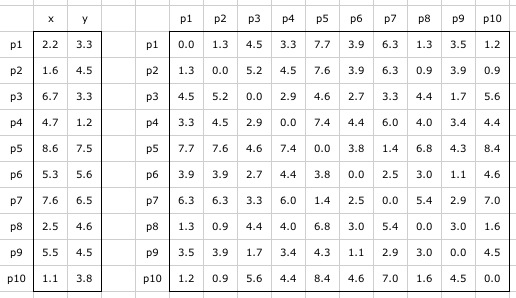
\includegraphics[width=4in]{eudistance.jpg}
\caption{A Euclidean distance matrix.}
\label{eudistance}
\end{table}

\subsection*{b}
% need to fix hierarchical clustering

% Distance is maximal between pairs

\Tree[.\{$p1,p2,p3,p4,p5,p6,p7,p8,p9,p20$\} 
	[.	[.	[.	[.	[.	[.	[.	[.	[.p2 ]
									[.p10 ]]
								[.	[.p8 ]]]]
						[.	[.	[.	[.p1	]]]]]
					[.	[.	[.	[.	[.p2	]]]]]]
	[.	[.	[.	[.	[.	[.	[.	[.	[.p5 ]]]
							[.	[.	[.p7 ]]]]]]]]]
	[.	[.	[.	[.	[.	[.	[.	[.	[.p6 ]]]]]
					[.	[.	[.	[.	[.p9 ]]]]]]
			[.	[.	[.	[.	[.	[.	[.p3 ]]]]]]]]	
					]]]]]]	

		
\subsection*{c} 
% Distance is minimal between pairs

\subsection*{d & e}
% k-means k=2.  P1,p2 are initial points

% k-means, k=2.  p9, p10 are initial points.

% write reflections

\section*{Question 5}
%need to remove \nlines and re-run.
\subsection*{1} The substrings were taken from crYsubset.fa.  I generated random 'slices' of this text of length 100 characters 500 times to generate the data below.


\subsection*{2}
\begin{figure}[h]
\centering
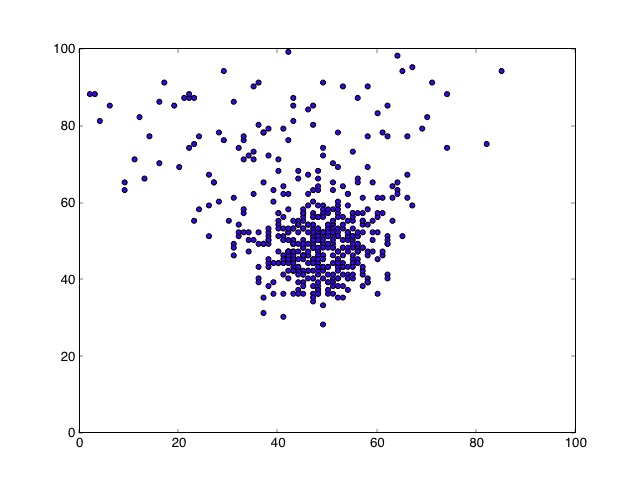
\includegraphics[width=4.5in]{scatter.jpg}
\caption{A scatter plot of runs in random 100 character subsequences, untransformed (x axis) and BW Transformed (y axis).}
\label{scatter}
\end{figure}

\subsection*{3}

\section*{Question 6: Programming exercise}

BWTSearch(BWTStringfilename, Querystr)

BWTStringfilename: filename which stores the B-W transformed string
QueryStr: Query String

Function should return comma separated locations of the query string in the original string. (Note: input file has B-W transformed string NOT original string). If query string is not found return -1

\end{document} 